\documentclass[letterpaper]{article} % DO NOT CHANGE THIS
\usepackage[submission]{aaai2027} % DO NOT CHANGE THIS
\usepackage[hyphens]{url} % DO NOT CHANGE THIS
\usepackage{graphicx} % DO NOT CHANGE THIS
\urlstyle{rm} % DO NOT CHANGE THIS
\def\UrlFont{\rm} % DO NOT CHANGE THIS
\usepackage{natbib} % DO NOT CHANGE THIS AND DO NOT ADD ANY OPTIONS TO IT
\usepackage{caption} % DO NOT CHANGE THIS AND DO NOT ADD ANY OPTIONS TO IT
\frenchspacing % DO NOT CHANGE THIS

\usepackage{amsmath,amssymb,amsthm}
\theoremstyle{plain}
\newtheorem{theorem}{Theorem}
\newtheorem{proposition}{Proposition}
\usepackage{booktabs}

\pdfinfo{
/TemplateVersion (2027.1)
}

\newcommand{\wcrit}{w_{\mathrm{crit}}}
\newcommand{\PT}{\mathrm{PT}}

\setcounter{secnumdepth}{2}

\title{Supplementary Material:\\Measuring Coordination-Collapse Boundaries in Reward-Mixed Cooperative MARL}

\author{
  Anonymous Submission
}
\affiliations{
  Paper under double-blind review
}

\begin{document}

\maketitle

\noindent This document contains the apparatus supporting the main paper: full experimental
setup and hyperparameters (\S\ref{sec:s_setup}), the complete loss-aversion sweep and
baseline reconciliation (\S\ref{sec:s_results}), the scoped mean-field derivation
(\S\ref{sec:s_mechanism}), the cross-environment and cross-algorithm detail
(\S\ref{sec:s_generalization}), both boundary-condition ablations (\S\ref{sec:s_ablations}),
the pre-registered signal-to-noise probe (\S\ref{sec:s_snr}), the exploration-noise ablation
(\S\ref{sec:s_entropy}), threshold robustness (\S\ref{sec:s_robustness}), notation
(\S\ref{sec:s_notation}), and a claim--evidence ledger (\S\ref{sec:s_ledger}). Section,
equation, and figure references to the main paper are by name. The supply-chain collapse label,
analysis code, and mechanism probes were fixed before execution; the anonymized code/data archive
included with the submission contains the corresponding records and scripts.

% =======================================================================
\section{Experimental Setup in Full}
\label{sec:s_setup}

\paragraph{Primary substrate.}
\texttt{NetworkManagement-v1} from or-gym~\citep{hubbs2020orgym}: a six-node multi-echelon
inventory network with Poisson demand ($\mu{=}20$) on the retail edge, 30-period episodes,
uniform lead times. Node~1 (retail-facing) follows a fixed demand-pull policy, stabilizing
the demand signal; nodes~2--6 are trained as cooperative PPO agents. Actions are
parameterized via a base-stock wrapper mapping each agent's continuous action to a target
inventory level $S\in[0,500]$, with order quantity $Q=\max(0,S-\mathrm{IP})$ where
$\mathrm{IP}$ is inventory position. The substrate extends prior DRL inventory work, the
Beer Distribution Game Dec-POMDP of \citet{oroojlooyjadid2022}, the multi-echelon A3C results
of \citet{gijsbrechts2022}, and single-echelon MARL~\citep{marlim2023}, to a six-node
network with per-node agents.

\paragraph{Algorithm and evaluation.}
The supply-chain learner is parameter-shared PPO (``IPPO'' in the shared-parameter sense): a single
shared actor--critic trained on the pooled per-node experience, with each node receiving its own
observation and acting through its own action indices, and decentralized execution. Each trained node
runs PPO~\citep{schulman2017ppo} on this shared-parameter MLP policy via
Stable-Baselines3~2.8.0~\citep{raffin2021sb3} with PettingZoo/SuperSuit
vectorization~\citep{terry2021pettingzoo,terry2020supersuit}; all hyperparameters are listed in
Table~\ref{tab:s_hparams} (values not set explicitly are SB3~2.8.0 defaults, enumerated there for
completeness). MAPPO uses the identical settings with a centralized (joint-state) critic. Evaluation
is deterministic over 10 episodes with 20 fixed seeds per condition; the 10-episode evaluation
estimates each trained policy's collapse label, while cross-run uncertainty (the bootstrap CIs) is
driven by the 20 training seeds, which the seed-paired bootstrap ($\S\ref{sec:s_controls}$) keeps
separate from evaluation noise.

\begin{table}[t]\centering\small
\caption{Full PPO/MAPPO hyperparameters (Stable-Baselines3 2.8.0). Only \texttt{n\_steps} and
\texttt{batch\_size} are set explicitly; the rest are SB3 defaults, listed for reproducibility.}
\label{tab:s_hparams}
\begin{tabular}{@{}p{0.40\linewidth}p{0.52\linewidth}@{}}
\toprule
Hyperparameter & Value \\
\midrule
Policy / value net & MLP, $2\times64$, $\tanh$ (shared params across nodes) \\
Centralized critic (MAPPO) & joint-state input, same $2\times64$ MLP \\
Learning rate & $3\times10^{-4}$ (constant) \\
Rollout length \texttt{n\_steps} & 128 \\
Minibatch size & 256 \\
Update epochs & 10 \\
Discount $\gamma$ & 0.99 \\
GAE $\lambda$ & 0.95 \\
Clip range & 0.2 \\
Value clip & none \\
Entropy coef. & 0.0 (except entropy ablation) \\
Value-loss coef. & 0.5 \\
Max grad norm & 0.5 \\
Advantage normalization & on \\
Parallel envs & 1 (one core/run; SuperSuit concat) \\
Policy init & SB3 default (orthogonal, gain $\sqrt2$) \\
Optimizer & Adam \\
\bottomrule
\end{tabular}
\end{table}

\paragraph{Computing infrastructure.}
All training is CPU-only (no GPU), one core per run on a Linux HPC cluster (PBS scheduler,
\texttt{ncpus}${=}1$; per-run walltimes of 3--12 hours scaling with the training horizon).
Software versions: Python with Stable-Baselines3~2.8.0, PettingZoo~1.26.1, SuperSuit~3.11.0,
Gymnasium~1.2.2, \texttt{mpe2}~1.1.0, PyTorch~2.12.0, NumPy~2.4.6, and pandas~3.0.3.

\paragraph{Experiment inventory.}
Table~\ref{tab:experiments} itemizes the primary supply-chain runs, total run count 5{,}064,
including the 150k/300k structural boundaries, the 450k/900k/600k horizon points behind the
metastability fit, the reward-transform decomposition and loss-aversion sweep, the finer
high-$\lambda$ grid, the entropy ablation, and the three reward-transform controls
(\S\ref{sec:s_controls}).

\begin{table}[t]
\centering
\caption{Primary supply-chain experiment inventory (same environment and algorithm unless noted;
$\alpha{=}\beta{=}1$ is the linear no-PT condition). Total 5{,}064 runs.}
\label{tab:experiments}
\small
\setlength{\tabcolsep}{3pt}
\begin{tabular}{@{}lp{0.28\linewidth}rrrr@{}}
\toprule
Exp & Purpose & $\lambda$ & $\alpha,\beta$ & Seeds & Runs \\
\midrule
A @150k & Struct.\ boundary & 1 & 1,1 & 20 & 220 \\
A @300k & Struct.\ boundary & 1 & 1,1 & 20 & 140 \\
C & Basin control & 1 & 1,1 & 12 & 144 \\
N & Null baseline & 1 & 1,1 & 20 & 180 \\
B-Red. & Reward-transf.\ decomp. & 1,3,7 & 0.88 & 20 & 300 \\
$\lambda$-sweep & Loss-av.\ law & 2,4,5,6 & 0.88 & 20 & 400 \\
T @450k & Metastability & 1 & 1,1 & 20 & 160 \\
T @900k & Metastability & 1 & 1,1 & 20 & 160 \\
T @600k & Metastability (curv.\ probe) & 1 & 0.88 & 20 & 140 \\
Entropy & SNR dissociation & 1 & 1,1 & 20 & 400 \\
High-$\lambda$ grid & Steep-cell resolution & 5,6,7 & 0.88 & 20 & 120 \\
Ctrl~A & Reference point ($4\times z_0$) & 1,3,7 & 0.88 & 20 & 1{,}200 \\
Ctrl~B & Scale match (RMS) & 1,3,7 & 0.88 & 20 & 600 \\
Ctrl~C & Reward units ($2\times$ loc/team) & 1,3,7 & 0.88 & 20 & 900 \\
\bottomrule
\end{tabular}
\end{table}

\paragraph{Basin control (rules out initialization).}
Exp~C rules out initialization as a collapse driver. Within-$w$ correlations between
$S_{\mathrm{init}}$ and converged $S$ are $-0.11$ ($w{=}0.5$), $-0.38$ ($w{=}0.85$), and
$-0.36$ ($w{=}1.0$), small to moderate and inconsistent with initialization dominating; the
collapsed/survived assignment is insensitive to where agents start.

\paragraph{Code and artifact.}
An anonymized code bundle accompanies this submission: the environment wrappers, all experiment
drivers and analysis scripts, the frozen collapse-label and control pre-registration records, and
the raw per-run result CSVs sufficient to regenerate every table and figure.

% =======================================================================
\section{Full Reward-Transform Sweep and Baseline Reconciliation}
\label{sec:s_results}

\paragraph{The recurring $\wcrit$ values.}
There is one structural null; the other recurring numbers are a horizon measurement of it and
a curvature \emph{result}, not independent baselines (Table~\ref{tab:baselines}).

\begin{table}[t]
\centering
\caption{The recurring $\wcrit$ values and the single role each plays.}
\label{tab:baselines}
\small
\begin{tabular}{lll}
\toprule
$\wcrit$ & Condition & Role \\
\midrule
$0.666$ & $\alpha{=}\beta{=}1$, 300k & structural null (main sweep) \\
$0.685$ & $\alpha{=}\beta{=}1$, 300k (Exp~N) & linear baseline, reproduced \\
$0.822$ & $\alpha{=}\beta{=}1$, 150k & null at shorter horizon \\
$0.585$ & $\alpha{=}\beta{=}0.88$, $\lambda{=}1$ & curvature result \\
\bottomrule
\end{tabular}
\end{table}

\paragraph{Full loss-aversion sweep.}
Table~\ref{tab:lambda_sweep} gives the complete $\lambda{=}1{\dots}7$ sweep with Firth penalized
fits. The increase is monotone up to estimation noise at the high-$\lambda$ plateau:
$\wcrit$ rises strictly from $\lambda{=}1$ to $\lambda{=}5$ then saturates near $0.84$--$0.85$
($\lambda{=}5,6$ statistically indistinguishable). At high loss aversion the transition is
very steep and falls between adjacent grid points (collapse fractions $1.00,1.00,1.00,0.55,
0.00$ at $w\in\{0.5,0.65,0.75,0.85,0.95\}$ for $\lambda{=}7$), so the boundary remains
identifiable (the $w{=}0.85$ cell is interior, $11/20$ collapsed) but the unpenalized MLE
slope diverges. Firth penalized logistic regression is stable here; all seven slopes reject a flat
relationship (max $p=1.5\times10^{-3}$) and the Firth $\wcrit$ matches the bootstrap to within $0.019$,
confirming the large unpenalized slopes at $\lambda{=}5,7$ were a fitting artifact, not
separation. The high-$\lambda$ plateau is a reward-transform saturation, not a $w{=}1$ ceiling
artifact: at $\lambda{=}7$ no evaluated runs collapse at $w{=}0.95$ (collapse fraction $0.00$),
consistent with the bounded affine law in which $\wcrit(\lambda)\to1$ only as
$\lambda\to\infty$. The $\lambda{\geq}5$ values in Table~\ref{tab:lambda_sweep} use a finer
$w\in\{0.80,0.90\}$ grid added specifically to resolve the steep transition; this places two
interior points across each high-$\lambda$ boundary and halves the CI widths
($0.038,0.033,0.024$ at $\lambda{=}5,6,7$) relative to the single $w{=}0.85$ cell, giving the
clean monotone $0.825\to0.835\to0.854$.

\begin{table}[t]
\centering
\caption{Full loss-aversion sweep ($\alpha{=}\beta{=}0.88$, 300k, 20 seeds/$(w,\lambda)$
cell, $n{=}100$ runs/$\lambda$). $\wcrit$ with bootstrap 95\% CIs; slope/$p$ from Firth
penalized logistic regression.}
\label{tab:lambda_sweep}
\small
\begin{tabular}{ccccc}
\toprule
$\lambda$ & $\wcrit$ & 95\% CI & Firth $b_1$ & $p$ \\
\midrule
1 & 0.585 & [0.545, 0.626] & $-14.7$ & $1.2\times10^{-6}$ \\
2 & 0.715 & [0.687, 0.745] & $-27.2$ & $4.4\times10^{-6}$ \\
3 & 0.774 & [0.751, 0.798] & $-29.7$ & $5.1\times10^{-6}$ \\
4 & 0.806 & [0.766, 0.841] & $-36.8$ & $5.5\times10^{-6}$ \\
5 & 0.825 & [0.806, 0.844] & $-53.1$ & $4.7\times10^{-4}$ \\
6 & 0.835 & [0.817, 0.850] & $-24.7$ & $2.5\times10^{-6}$ \\
7 & 0.854 & [0.837, 0.871] & $-43.1$ & $1.5\times10^{-3}$ \\
\bottomrule
\end{tabular}
\end{table}

\paragraph{Metastability under matched curvature.}
The exploratory 600k metastability probe (Table~\ref{tab:experiments}, T~@600k) uses
$\alpha{=}\beta{=}0.88$, which shifts $\wcrit$ left by $0.100$, so its collapse fractions are partly
curvature-deflated. The main-text four-horizon slide is measured at matched $\alpha{=}\beta{=}1$ and
is therefore already curvature-free; for a direct comparison at 600k under $\alpha{=}\beta{=}1$
(Exp~0b, 20 seeds), $P(\mathrm{collapse}\mid w{=}0.6)=0.35$ and $P(\mathrm{collapse}\mid w{=}0.7)=0.20$,
versus $0.80$ and $0.40$ at 300k: the horizon slide holds with curvature held constant, confirming
it is not a curvature artifact.

\paragraph{The metastable slide generalizes.}
The horizon dependence is not a supply-chain artifact. We ran dedicated horizon sweeps under
centralized-critic MAPPO on both transfer environments. On MPE Cooperative Navigation,
$\wcrit$ falls $0.82\to0.68$ as the horizon grows $2\mathrm{M}\to8\mathrm{M}$ env steps (slide
$+0.14$); on Level-Based Foraging it falls $0.33\to0.20$ over $1\mathrm{M}\to4\mathrm{M}$
(slide $+0.13$), each with non-overlapping bootstrap intervals at the endpoints. Both match
the supply-chain direction (boundary slides left with more training), so the metastability
result (like the loss-aversion direction) holds across environments and algorithms, not just
on the primary substrate.

\paragraph{The four-horizon log-linear fit.}
On the supply chain we measured $\wcrit$ at four matched risk-neutral horizons
(Table~\ref{tab:horizons}). The four points fall on a log-linear law $\wcrit=2.44-0.138\ln T$
(RMSE $0.027$), the Kramers escape-time prediction that $\wcrit$ falls as $-\ln T$ toward the
deterministic floor $\wcrit^0=c/(c+g)$. All four CI widths are ${\le}0.073$, and the
300k/450k/900k widths are ${\le}0.054$, so the law is a fitted four-point relationship, not a
two-point extrapolation.

\begin{table}[t]
\centering \small
\caption{Matched risk-neutral horizons ($\alpha{=}\beta{=}1$, $\lambda{=}1$). $\wcrit$ with
bootstrap 95\% CIs; the four points fit $\wcrit=2.44-0.138\ln T$ at RMSE $0.027$.}
\label{tab:horizons}
\begin{tabular}{lcc}
\toprule
$T$ (env steps) & $\wcrit$ & 95\% CI \\
\midrule
150k & 0.822 & [0.785, 0.858] \\
300k & 0.666 & [0.635, 0.694] \\
450k & 0.622 & [0.603, 0.641] \\
900k & 0.573 & [0.547, 0.598] \\
\bottomrule
\end{tabular}
\end{table}

\subsection{Is collapse a distinct regime? Continuous-metric distributions}
\label{sec:s_bimodality}
A fitted 50\% crossing exists whenever the binary label varies monotonically with $w$, so the
substantive question is whether there are genuinely distinct behavioral regimes or a continuous
degradation. Figure~\ref{fig:s_bimodality} plots the continuous metric per run across $w$ at
$\lambda{=}1$. A point-estimate bimodality coefficient a hair above a
descriptive rule-of-thumb, with no uncertainty and no formal test, is not sufficient evidence for a
distinct dynamical regime; we address this directly.

\paragraph{Bootstrap CI and Hartigan's dip test.} For each substrate and $w$ we compute a bootstrap
95\% CI on Sarle's bimodality coefficient ($2000$ resamples) and Hartigan's dip test against a
unimodal null (\texttt{experiments/bimodality\_significance.py}). On the supply chain, the mean
base-stock $\bar S$ shows the same qualitative pattern as before (runs cluster near $\bar S\!\approx\!0$
or in $[45,320]$, e.g.\ $8/20$ runs at $\bar S{=}0$ at $w{=}0.65$; coefficient $0.59,0.57$ at
$w{=}0.65,0.75$), but the bootstrap CI is wide and straddles $0.555$ at every $w$ (e.g.\
$[0.43,0.78]$ at $w{=}0.65$, $[0.45,0.74]$ at $w{=}0.75$), and the dip test does not reject unimodality
at any $w$ ($p\ge0.30$, $n{=}20$/cell). On LBF, the raw team-return dip test is nominally significant
at high $w$ ($p=0.014,0.002,0.002$ at $w{=}0.75,0.85,0.95$), which would seem to favor bimodality on
the substrate we had called a smooth continuum. Inspecting the raw values shows this is a ceiling
artifact: $7$--$8$ of $40$ runs per cell saturate exactly at the metric's upper bound. Excluding
ceiling-clipped runs removes the significance at every $w$ ($p\ge0.11$).

\paragraph{Conclusion.} Neither substrate clears a formal multimodality test at our sample sizes ($n{=}20$
per supply-chain cell, $n{=}40$ per LBF cell). We therefore withdraw the ``genuine attractor'' claim for
the supply chain and describe ``collapse'' uniformly, on both substrates, as a threshold-defined
behavioral crossing rather than a confirmed distinct regime. This also means the ``metastable escape''
framing (\S\ref{sec:s_mechanism}) should be read as describing the horizon-dependence of a threshold
crossing, not basin-level escape dynamics; we do not have dwell-time, escape-time, or hysteresis
evidence for either substrate. Distinguishing a true attractor from a steep continuum would need larger
per-cell $n$, unbounded (non-ceiling-clipped) continuous metrics, and trajectory-level probes; we leave
this to future work.

\begin{figure}[t]
 \centering
 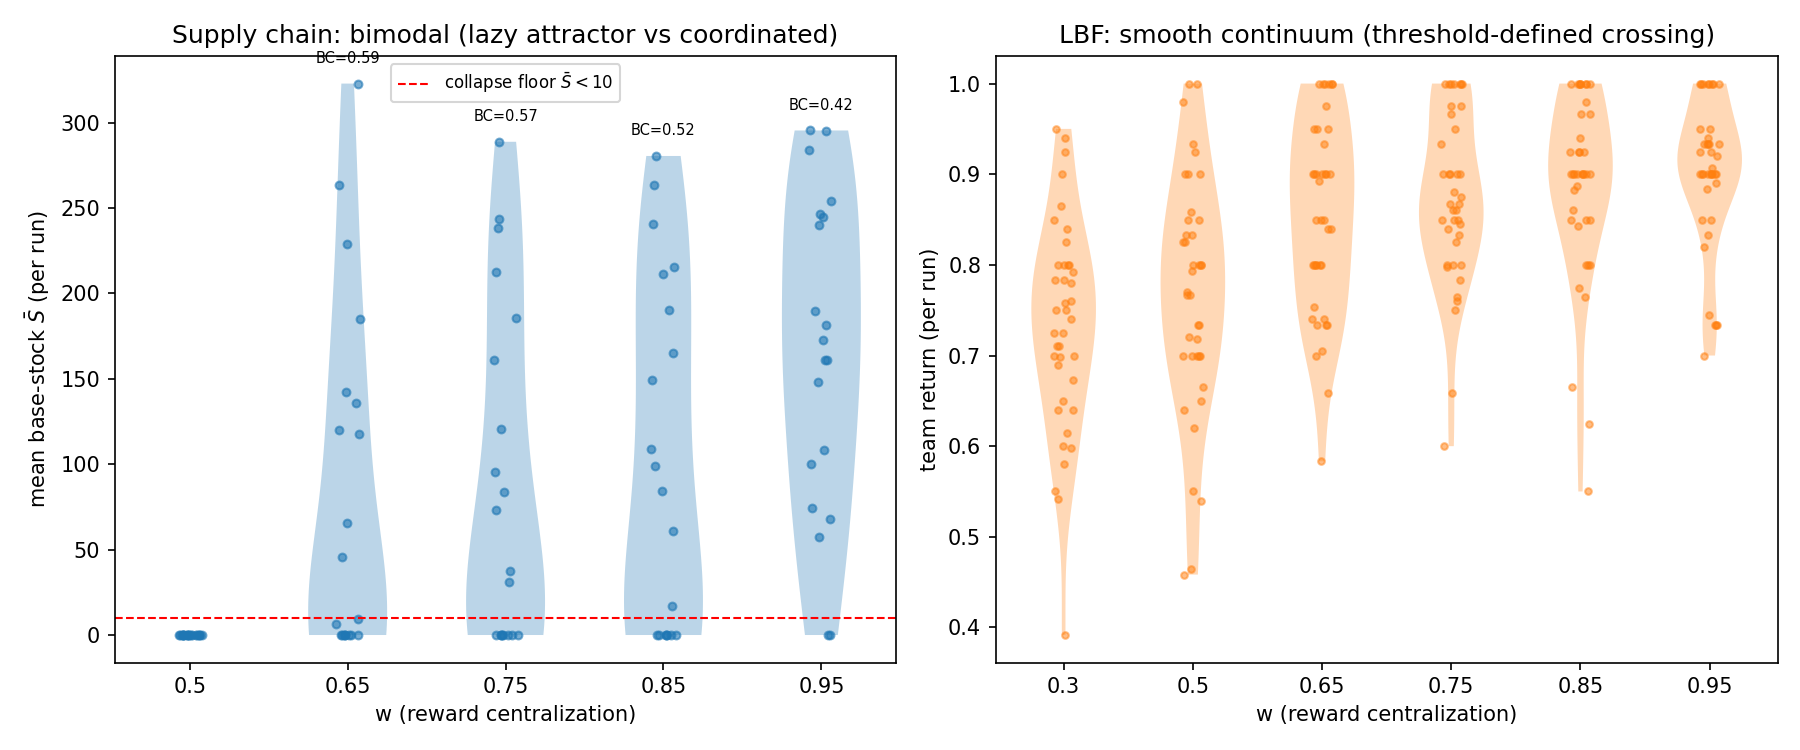
\includegraphics[width=\columnwidth]{Figures/bimodality_supply_vs_lbf}
 \caption{Per-run continuous metric across $w$ ($\lambda{=}1$). Left: supply-chain mean base-stock
  $\bar S$ shows the same qualitative clustering near $\bar S\!\approx\!0$ vs.\ coordinated, with an
  empty gap; the collapse floor $\bar S<10$ is dashed; a dip test does not reject unimodality at any
  $w$ (\S\ref{sec:s_bimodality}). Right: LBF team return, with the ceiling-clipped runs responsible for
  the raw dip-test signal visible as the pileup at $1.0$.}
 \label{fig:s_bimodality}
\end{figure}

\medskip\noindent The derived affine law~\eqref{eq:wcrit_lambda} and its out-of-sample fit
(RMSE $0.014$ across all seven points) are shown and discussed in the main paper; the
derivation of its form is given in \S\ref{sec:s_mechanism} below.

\subsection{Estimator robustness (link function and nonparametric fit)}
\label{sec:s_estimator}
We refit every $\wcrit$ under three estimators: logistic (primary), probit, and isotonic regression
(monotone-decreasing in $w$, no functional form). Across all $\lambda$ and all three environments
the estimates agree to $\le0.02$, and the isotonic $\wcrit$ (which assumes only monotonicity) tracks
the logistic to within one grid step, so the reported location and its CI are not consequences of the
logistic link. On the primary supply-chain sweep the logistic/Firth and isotonic $\wcrit(\lambda)$
coincide at $\{0.585/0.575,\,0.774/0.786,\,0.854/0.859\}$ for $\lambda\in\{1,3,7\}$, and the
$\lambda{=}1{\to}7$ shift is $+0.269$ (logistic/Firth) versus $+0.284$ (isotonic); McFadden pseudo-$R^2$
for the logistic fits is $\ge0.6$ at every interior cell. The same agreement holds on MPE and LBF,
where the seed-paired $\lambda$-shift CI excludes zero under all three estimators.

% =======================================================================
\section{Mean-Field Mechanism: Scope and Derivation}
\label{sec:s_mechanism}

This section gives the mechanism underlying the sign-level claims in the main paper. Its scope is
deliberately narrow. The derivation is a mean-field account for the primary supply-chain PPO
setting, where agents use continuous base-stock actions and the reward-mixing dial $w$ creates a
local--global incentive conflict. It is not a closed-form derivation of the numerical value of
$\wcrit$. The empirical boundary remains calibrated by the fitted collapse curve; the mechanism offers
a candidate account of why a boundary exists, why its position slides with the training horizon, and
why loss aversion raises it under a local signal-to-noise premise checked on that substrate. We do not
have distributional or basin-level evidence for a distinct regime (\S\ref{sec:s_bimodality}), so
``sharp'' should be read as ``well-estimated,'' not as evidence of a sudden dynamical transition.

\subsection{Reward transform and policy-mean dynamics}
Each trained node $i$ receives the reward-mixed scalar
\begin{equation}
 z_i(a)=(1-w)\ell_i(a_i,a_{-i})+wG(a),\qquad G(a)=\sum_j \ell_j(a),
 \label{eq:blend}
\end{equation}
where $\ell_i$ is the local profit of node $i$ and $G$ is system profit. The prospect-theoretic
value transform used in the experiments is
\begin{equation}
 v(z)=
 \begin{cases}
 z^\alpha, & z\ge 0,\\
 -\lambda(-z)^\beta, & z<0.
 \end{cases}
\end{equation}
Thus the shaped training signal is $r_i^{\mathrm{PT}}=v(z_i)$. We do not model probability
weighting in this paper; the experimental transform consists only of value-function curvature
$(\alpha,\beta)$ and loss aversion $\lambda$.

For the continuous-action PPO supply-chain substrate, let $m_i$ denote the mean of agent $i$'s
Gaussian base-stock policy. Around a slowly varying policy state, the stochastic PPO update of
$m_i$ can be approximated by the diffusion
\begin{equation}
 \mathrm{d}m_i
 =
 F_i(m;w,\alpha,\beta,\lambda)\,\mathrm{d}t
 +
 \sqrt{\Sigma_i(m;w,\alpha,\beta,\lambda)}\,\mathrm{d}W_i ,
 \label{eq:langevin}
\end{equation}
where $F_i$ is the expected policy-mean drift and $\Sigma_i>0$ is the variance of the stochastic
update. We use $F$ only for drift and $\Sigma$ only for diffusion variance. Constant factors in the
diffusion convention, such as whether one writes $\sqrt{\Sigma}$ or $\sqrt{2\Theta}$, are absorbed
into the critical signal-to-noise threshold below and do not affect any sign claim.

\subsection{The local--global incentive conflict}
The primary supply-chain substrate has the incentive asymmetry required for a collapse boundary.
Along the base-stock direction, increasing an upstream node's stock is locally costly because it
increases holding and procurement costs, but globally beneficial because it prevents downstream
stockouts. A finite-difference probe of the substrate gives the local signs
\begin{equation}
 \partial_a \mathbb{E}[\ell_i]\approx -c,\qquad
 \partial_a \mathbb{E}[G]\approx +g,\qquad c,g>0.
\end{equation}
Ignoring the prospect transform and stochastic-update variance, the cooperative component of the
policy-mean drift has the form
\begin{equation}
 F_0(w)=\eta\{wg-(1-w)c\}.
 \label{eq:drift}
\end{equation}
The deterministic zero-drift crossing is therefore
\begin{equation}
 \wcrit^0=\frac{c}{c+g}.
\end{equation}
This is not the empirical boundary measured in the paper. It is only the low-noise,
infinite-horizon floor toward which the finite-horizon boundary can move. At finite horizon,
stochastic updates and basin geometry make the operative boundary a signal-to-noise crossing, not
merely the point where the deterministic drift changes sign.

\subsection{Collapse as failure to escape the lazy basin}
Let $x\in[0,1]$ be a latent order parameter measuring progress from the lazy basin toward
coordinated behavior. We do not claim that $x$ is directly observed in the experiments. It is a
macroscopic coordinate used to describe the basin-level dynamics:
\begin{equation}
 \mathrm{d}x_t = F(x_t,w,\lambda)\,\mathrm{d}t
 + \sqrt{\Sigma(x_t,w,\lambda,N)}\,\mathrm{d}W_t .
 \label{eq:sde}
\end{equation}
Here $F$ is the effective drift toward coordination and $\Sigma$ is the stochastic-update variance.
Let $\tau_{L\to C}(w,\lambda)$ denote the mean first-passage time to escape the lazy basin and
reach the coordinating basin.

This convention fixes the direction of the argument. A run is collapsed at training horizon $T$
when it has not escaped the lazy basin by the end of training:
\begin{equation}
 \text{collapse at horizon }T
 \quad\Longleftrightarrow\quad
 \tau_{L\to C}(w,\lambda)>T
\end{equation}
up to the usual stochastic first-passage variability. The empirical midpoint
$\wcrit^{\mathrm{Emp}}(T,\lambda)$ is the value of $w$ at which the fitted collapse probability
equals $1/2$, equivalently the finite-horizon crossing where the typical escape time is on the
order of $T$.

Increasing $w$ strengthens the cooperative global component of the reward, so it decreases
$\tau_{L\to C}$. Increasing loss aversion weakens the effective escape signal relative to update
noise in the loss domain, so it increases $\tau_{L\to C}$. Therefore a larger $w$ is required to
reach the same fixed-horizon crossing when $\lambda$ increases.

\subsection{Signal-to-noise form of the boundary}
The quantity that matters near the boundary is not drift alone, but escape signal-to-noise. Define
the local escape SNR
\begin{equation}
 \mathcal{S}(w,\lambda)
 =
 \frac{F_{\mathrm{esc}}(w,\lambda)}
 {\sqrt{\Sigma_{\mathrm{esc}}(w,\lambda)}} ,
 \label{eq:escape_snr}
\end{equation}
where $F_{\mathrm{esc}}$ and $\Sigma_{\mathrm{esc}}$ denote the effective drift and update variance
on the escape interval from the lazy basin to the coordinating basin. The finite-horizon boundary
is the crossing
\begin{equation}
 \mathcal{S}(w,\lambda)\approx \kappa_T ,
\end{equation}
where $\kappa_T$ is a horizon-dependent critical value. Longer training horizons require a smaller
escape SNR, so $\wcrit(T)$ decreases with $T$. This gives the metastable interpretation of the
observed horizon slide: at any fixed training budget the boundary is well-defined, but additional
training can rescue some policies below the shorter-horizon boundary.

Equivalently, in the one-dimensional diffusion approximation, Kramers' first-passage form gives
\begin{equation}
 \tau_{L\to C}(w,\lambda)
 \asymp
 \tau_0
 \exp\{\Delta U_{L\to C}(w,\lambda)\},
 \label{eq:barrier}
\end{equation}
where $\Delta U_{L\to C}$ is the effective quasi-potential barrier for leaving the lazy basin.
Larger escape SNR lowers this barrier and shortens $\tau_{L\to C}$; lower escape SNR raises the
barrier and lengthens $\tau_{L\to C}$. The numerical value of $\Delta U_{L\to C}$ depends on the
unobserved covariance structure of PPO updates, so the mechanism does not produce a closed-form
numerical $\wcrit$.

\subsection{Sign propagation under a checked local premise}
The sign claim used in the main paper is conditional on a local premise, checked on the
supply-chain substrate, about how $w$ and $\lambda$ affect the escape SNR.

\paragraph{Premise.}
On the supply-chain PPO escape interval,
\begin{equation}
 \partial_w \mathcal{S}(w,\lambda)>0,\qquad
 \partial_\lambda \mathcal{S}(w,\lambda)<0.
\end{equation}
The first inequality states that increasing centralization strengthens the escape signal. The
second states that increasing loss aversion lowers the effective escape signal-to-noise ratio. This
second effect may arise through drift, diffusion, or both: loss aversion changes the transformed
reward landscape in the loss domain and can increase stochastic update variance relative to the
cooperative escape signal. We therefore state the premise at the SNR level rather than identifying
it with drift alone.

\begin{proposition}[Loss aversion raises the empirical boundary]\label{thm:sign}
Assume the local SNR premise above and assume the mean escape time $\tau_{L\to C}$ is strictly
decreasing in $\mathcal{S}$. Then, at fixed training horizon $T$,
\begin{equation}
 \frac{\mathrm{d}\wcrit^{\mathrm{Emp}}}{\mathrm{d}\lambda}>0 .
\end{equation}
\end{proposition}
\begin{proof}
The empirical boundary is the fixed-horizon crossing
\begin{equation}
 \tau_{L\to C}(w,\lambda)=T .
\end{equation}
Since $\tau_{L\to C}$ decreases with escape SNR and $\partial_w\mathcal{S}>0$, we have
$\partial_w \tau_{L\to C}<0$. Since $\partial_\lambda\mathcal{S}<0$, increasing loss aversion
lengthens the lazy-to-coordination escape time: $\partial_\lambda \tau_{L\to C}>0$. Applying the
implicit function theorem to $H(w,\lambda)=\tau_{L\to C}(w,\lambda)-T=0$ gives
\begin{equation}
 \frac{\mathrm{d}\wcrit^{\mathrm{Emp}}}{\mathrm{d}\lambda}
 =
 -\frac{\partial_\lambda \tau_{L\to C}}
 {\partial_w \tau_{L\to C}}
 >0 .
\end{equation}
The proposition proves only the direction. Its magnitude depends on the unobserved diffusion and
basin geometry, which is why the empirical boundary is measured rather than predicted in closed
form.
\end{proof}

\subsection{Curvature is scoped to the primary substrate}
The same SNR language explains why value-function curvature and loss aversion can move the boundary
in opposite directions on the primary supply-chain PPO substrate. In that setting, concave value
curvature $(\alpha,\beta<1)$ compresses reward variation and empirically raises the escape SNR
relative to the linear transform, lowering $\wcrit$. Loss aversion magnifies the loss-domain
component and lowers the escape SNR, raising $\wcrit$.

This curvature sign is not claimed to be universal. It is a primary-substrate result. The transfer
experiments show that the loss-aversion direction generalizes, while the curvature sign and exact
functional form are substrate-specific. Thus the mechanism supports the supply-chain decomposition
and the sign of the loss-aversion shift, but it does not claim a global curvature theorem for all
cooperative MARL tasks.

\subsection{Affine loss-aversion law on the supply-chain substrate}
The supply-chain PPO sweep is additionally summarized by a bounded one-parameter law after anchoring
the baseline. At $\lambda=1$, the curvature baseline fixes the ratio $g/c$ through
\begin{equation}
 \wcrit(1)=\frac{1}{1+g/c}.
\end{equation}
Loss aversion scales only the loss-domain share of the marginal escape incentive. Writing that
share as $\rho\in[0,1]$, define
\begin{equation}
 \phi(\lambda)=1+\rho(\lambda-1).
\end{equation}
The resulting bounded form is
\begin{equation}
 \wcrit(\lambda)=\frac{\phi(\lambda)}{\phi(\lambda)+g/c}.
 \label{eq:wcrit_lambda}
\end{equation}
This is not a free closed-form prediction of the numerical boundary. The baseline anchors $g/c$,
and $\rho$ is one additional calibrated parameter. The useful content is that the form is monotone,
bounded, and saturating. Fitting $\rho$ on $\lambda\in\{3,7\}$ and holding out $\lambda\in\{2,4,5,6\}$
gives $\wcrit^{\mathrm{pred}}=\{0.585,0.696,0.761,0.802,0.832,0.854,0.870\}$ against
$\wcrit^{\mathrm{meas}}=\{0.585,0.715,0.775,0.805,0.820,0.835,0.854\}$ (Figure~\ref{fig:affine}):
held-out RMSE $0.014$, all-seven RMSE $0.013$; leave-one-out fits keep $\rho\in[0.59,0.64]$
($\rho=0.63$ on the full $\lambda\in\{3,7\}$ calibration).

Two caveats bound this. First, the held-out $\lambda$ share environment, algorithm, and horizon with
the calibration points, so this is an interpolation check within one sweep, not out-of-distribution
validation, and a weak one: held-out RMSE ($0.014$) is on the same scale as the held-out points' own
bootstrap CI half-widths ($0.017$--$0.027$), near the measurement noise floor. We treat the form as a
parsimonious summary, not a validated law. Second, the $\rho\in[0,1]$ bound is slack here
($\rho{=}0.63$) but binds on LBF, where the affine form misfits at RMSE $0.15$: the loss-aversion
\emph{sign} transfers there but this specific functional form does not.

\begin{figure}[t]
 \centering
 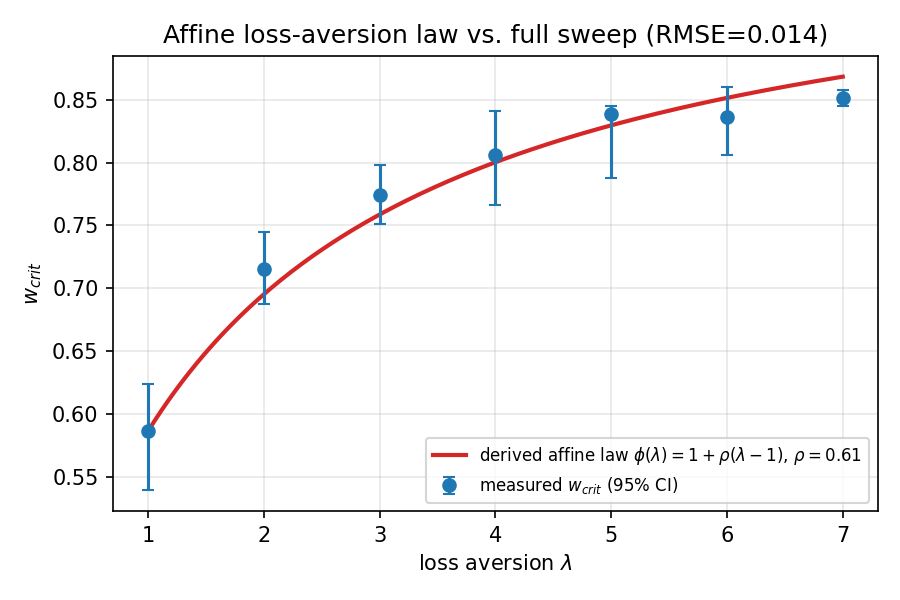
\includegraphics[width=0.82\columnwidth]{Figures/affine_law_7pt}
 \caption{The one-parameter saturating summary (line, $\rho{=}0.63$ after anchoring $g/c$ at
  $\lambda{=}1$) against measured $\wcrit(\lambda)$ (points, bootstrap 95\% CIs). Held-out RMSE on
  $\lambda\in\{2,4,5,6\}$ is $0.014$; all-seven RMSE is $0.013$. An interpolation check within one
  sweep, not out-of-distribution validation.}
 \label{fig:affine}
\end{figure}

The affine law is therefore a single-substrate mechanism summary. It is not claimed to transfer to
LBF or MPE, where the absolute levels, curvature sign, and functional form differ.

\begin{table}[t]
\centering
\caption{What the mean-field mechanism claims after separating modeled signs from calibrated
quantities.}
\label{tab:ledger_full}
\small
\begin{tabular}{p{0.28\linewidth}p{0.62\linewidth}}
\toprule
\textbf{Category} & \textbf{Claim} \\
\midrule
\textbf{Modeled, not fitted} &
On the primary supply-chain PPO substrate: increasing $w$ raises escape SNR; increasing $\lambda$
lowers escape SNR; therefore loss aversion raises $\wcrit$. Finite-horizon escape gives sharpness
and a leftward horizon slide. \\
\midrule
\textbf{Empirically confirmed} &
Resolved (non-flat, tightly-estimated) threshold crossing; horizon slide; loss-aversion direction
across SC, MPE, and LBF; entropy-noise dissociation where injected noise is binding. \\
\midrule
\textbf{Calibrated/fitted} &
Absolute $\wcrit$; diffusion scale; $g/c$ from the baseline; one additional affine-law parameter
$\rho$ after baseline anchoring. \\
\midrule
\textbf{Not claimed} &
Closed-form numerical $\wcrit$; universal curvature sign; transfer of the affine law beyond the
supply-chain PPO substrate; direct observability of the latent order parameter. \\
\bottomrule
\end{tabular}
\end{table}

% =======================================================================
\section{Generalization Detail}
\label{sec:s_generalization}

\subsection{Cross-environment: MPE Cooperative Navigation}
Three agents cover three landmarks in a continuous 2-D arena (discrete actions, 50-step
episodes). The locally rational action under the herding incentive is to stay near
teammates, collectively disastrous, as agents cluster and no landmark is covered. We set
\texttt{local\_ratio}${=}0$ so the raw reward is the pure global team score; the herding term
is defined by our wrapper. Collapse is per-step landmark occupancy (fraction of landmarks
within a fixed radius of some agent), an evaluation metric invariant to reward scale and so
unaffected by the reward transform. Unlike the supply chain (per-agent incentives), MPE's
coordination reward is shared-global, which under independent learners confounds reward-transform
collapse with credit-assignment failure; we therefore train MPE with centralized-critic
MAPPO~\citep{yu2022surprising,lowe2017multi}, implemented as Stable-Baselines3 PPO with a
centralized (joint-state) critic policy so the optimizer matches the supply-chain PPO. The herding
wrapper defines each agent's local reward as
\begin{equation}
r_i^{\mathrm{local}}=-\,\kappa_{\mathrm{herd}}\cdot
\tfrac{1}{N-1}\sum_{j\ne i}\lVert p_i-p_j\rVert_2,\qquad \kappa_{\mathrm{herd}}=4,
\end{equation}
with $p_i$ agent $i$'s position; the raw env uses \texttt{local\_ratio}${=}0$ so $r^{\mathrm{global}}$
is the pure team score. The scale $\kappa_{\mathrm{herd}}{=}4$ places the theoretical indifference
point at $w^\ast\approx0.62$ (from $(1{-}w)\,\overline{r_{\mathrm{herd}}}=w\,\overline{r_{\mathrm{global}}}$
with measured means $42.3$ and $26.3$), so the no-transform boundary is interior ($\wcrit{=}0.74$);
it was fixed before the $\lambda$-sweep. We ran the full $\lambda$-sweep (1{,}760 runs, 20 seeds/cell;
Figure~\ref{fig:mpe_lambda_curves}). The loss-aversion effect replicates, $\wcrit$ rises
$0.78\to0.89$ over $\lambda{=}1\to7$, rising in envelope but non-monotone at intermediate
$\lambda$, excess $+0.158$ $[0.108,0.212]$ at $\lambda{=}7$ and $+0.101$ $[0.055,0.150]$ at
$\lambda{=}3$ (matching the supply chain's $+0.089$). The curvature effect does \emph{not}
replicate ($+0.042$ $[-0.009,0.092]$, opposite in sign), and the affine form fits MPE only to
RMSE $0.05$.

\begin{figure}[t]
 \centering
 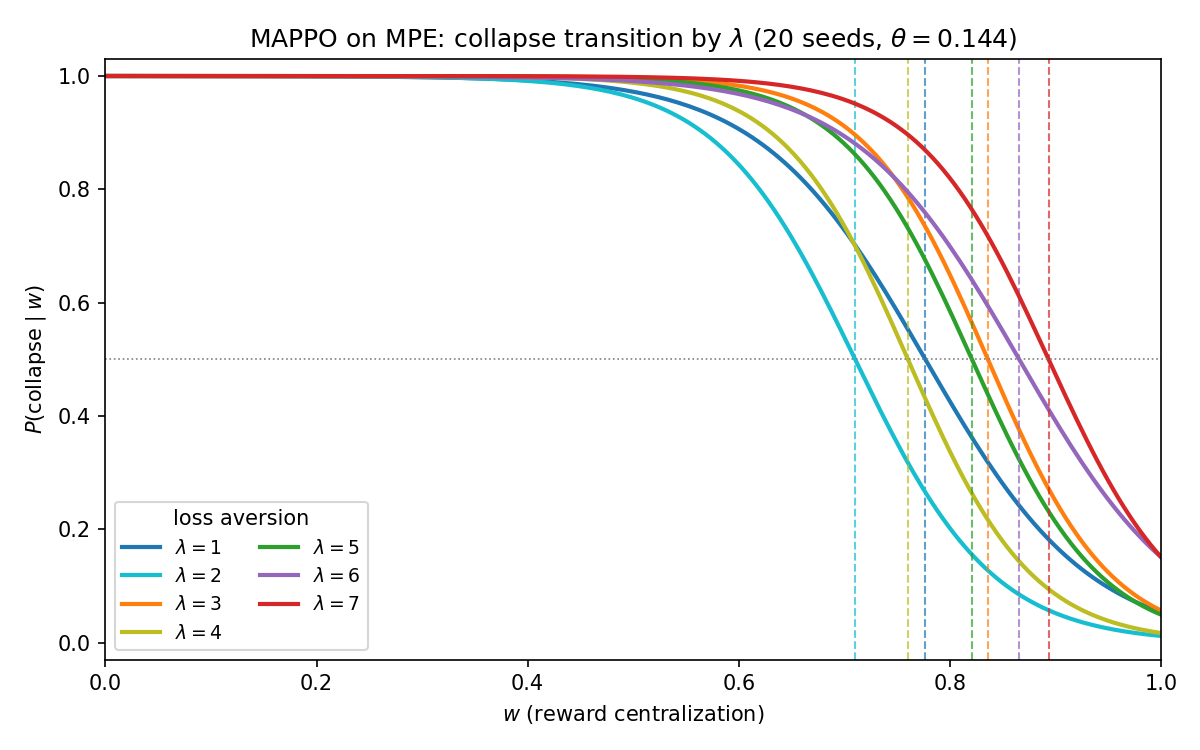
\includegraphics[width=0.9\columnwidth]{Figures/mappo_mpe_lambda_curves}
 \caption{MAPPO on MPE Cooperative Navigation: fitted $P(\mathrm{collapse}\mid w)$ for
  $\lambda{=}1,\dots,7$ ($\alpha{=}\beta{=}0.88$, centralized critic, collapse = landmark
  occupancy below $\theta{=}0.144$). The family shifts rightward with $\lambda$, the same
  loss-aversion signature, under a different environment and algorithm.}
 \label{fig:mpe_lambda_curves}
\end{figure}

\subsection{A third environment: Level-Based Foraging}
LBF~\citep{christianos2020shared} has a public-goods incentive: agents pay an effort cost to
load food cooperatively, so the locally rational action is to free-ride. Concretely LBF is
\texttt{Foraging-5x5-2p-2f-v3}: a $5\times5$ grid, $2$ players, $2$ foods, with per-agent rewards
equal to each loader's share of a food (normalized so loading all foods sums to a fixed total); the
$2$-player $5\times5$ configuration is deliberately small so the $w{=}1$ team-summed reward remains
learnable. Natively discrete, unrelated to logistics or navigation, trained under centralized-critic
MAPPO (matching MPE so only the environment varies), full $\lambda$-sweep, same collapse-midpoint
criterion: the team return (sum of per-agent shares over an evaluation episode) below
$\theta{=}0.626$, the calibrated collapsed-versus-coordinated midpoint (1{,}600 runs). The risk-neutral null is low and tight ($\wcrit\approx0.08$); curvature moves it
\emph{right} by $+0.18$ (opposite to the supply chain). Loss aversion drives $\wcrit$ from
$0.26$ at $\lambda{=}1$ to $0.83$ at $\lambda{=}4$, monotone with non-overlapping endpoint CIs
(the pre-registered criterion), robust to the collapse threshold. For $\lambda\geq5$ the
boundary saturates against the centralization ceiling: the logistic $\wcrit$ extrapolates to
$w\geq1$ (outside the measured $w\in[0,0.95]$ grid), so these points are \emph{not} interior
estimates and we label them exploratory in the precise sense that their $\wcrit$ lies beyond the
range any run samples, their location is bounded below by $0.95$ but not upper-bounded by the data.
An added intermediate level $w{=}0.90$ tightens the mid-$\lambda$ estimates and confirms the
saturation, but does not bring the $\lambda\geq5$ crossings inside the grid. The supply chain's affine law does not transfer: with $\gamma$ fixed
from $\lambda{=}1$, the best-fit slope saturates at its bound and misfits LBF by RMSE $0.15$,
converting the form's substrate-specificity from assertion to measured result.

\subsection{Transfer-environment label calibration}
\label{sec:s_transfer_calib}
Both transfer thresholds were fixed by the same collapsed-versus-coordinated midpoint rule used for
the supply chain, and, critically, set from the $\lambda{=}1$ (untreated) endpoints \emph{before}
the loss-aversion sweep, so no threshold was chosen after seeing a treatment outcome. For MPE, the
collapse metric is per-step landmark occupancy; at the calibration endpoints the coordinated regime
($w$ high) occupies $\approx0.28$ of landmarks and the free-riding regime ($w{=}0$) $\approx0.05$, and
$\theta=0.144$ is their midpoint. For LBF, the metric is episode team return; the coordinated
(null, high-$w$) and collapsed (high-$\lambda$, low-$w$) regimes bracket the midpoint at
$\theta=0.626$. The occupancy and return metrics are evaluation quantities invariant to the reward
transform, so the label does not move with $\lambda$. The direction result is additionally reported as
robust to the threshold: on LBF the monotone $\lambda$-rise holds under $\pm$ perturbations of
$\theta$, and the pre-registered endpoint criterion (non-overlapping $\lambda{=}1$ vs.\ last-interior
CIs) does not depend on the midpoint value.

\subsection{Cross-algorithm: MAPPO on the supply chain}
To isolate the algorithm from the environment, we re-run the full sweep on the \emph{identical}
substrate, grid, seeds, label, and hyperparameters, changing only the learner from independent
PPO to centralized-critic MAPPO (700 runs; Figure~\ref{fig:mappo_curves}). $\wcrit$ rises
$0.796\,[0.742,0.860]$ at $\lambda{=}1$ to $0.889\,[0.856,0.917]$ at $\lambda{=}7$, monotone
from $\lambda{=}2$ ($0.747,0.795,0.800,0.851,0.861,0.889$), endpoint CIs non-overlapping. The
direction generalizes while the absolute level does not: MAPPO sits above PPO at low $\lambda$
(most visibly $\lambda{=}1$, $0.796$ vs $0.585$, where MAPPO's transition is shallow and the
estimate noisier), converging by $\lambda\geq4$ ($|\Delta\wcrit|\leq0.04$).

\begin{figure}[t]
 \centering
 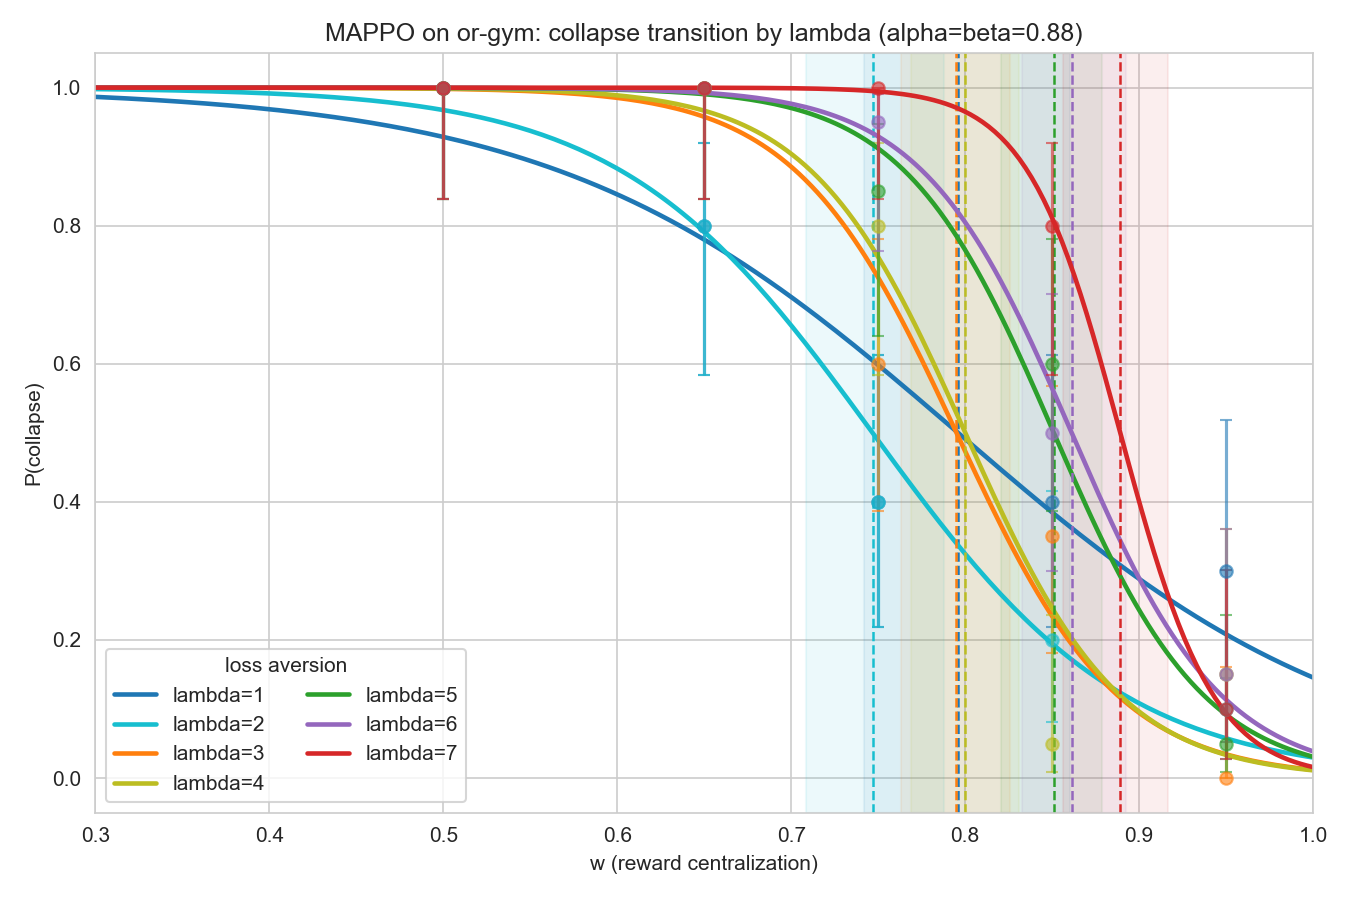
\includegraphics[width=0.9\columnwidth]{Figures/mappo_orgym_collapse_curves}
 \caption{Centralized-critic MAPPO on the supply chain: $P(\mathrm{collapse}\mid w)$ for
  $\lambda{=}1,\dots,7$ (700 runs). As under PPO, the family shifts rightward with loss
  aversion, confirming the effect is not an artifact of independent PPO.}
 \label{fig:mappo_curves}
\end{figure}

\subsection{Downstream-minority cascade (figure)}
\label{sec:s_cascade}
Figure~\ref{fig:s_cascade} accompanies the minority-node analysis in the main paper
(\S``A Single Downstream Node Can Nearly Set the Boundary''): panel~(a) is the position sweep
(one $\lambda{=}7$ node at each network position) and panel~(b) the single-downstream-node
dose-response. The experiment holds the environment, PPO configuration, collapse label, $w$-grid,
and estimator identical to the main homogeneous sweep. Bootstrap 95\% CIs (Firth $\wcrit$, seed
resampling, $2{,}000$ replicates, $n{=}20$ seeds/position) for panel (a):
node\_2 (retail-adjacent) $0.863\,[0.846,0.880]$; node\_3 (retail-adjacent)
$0.800\,[0.780,0.820]$; node\_5 (sole supplier to the dominant downstream node)
$0.797\,[0.740,0.857]$; node\_6 (split-path) $0.726\,[0.682,0.769]$; node\_4 (split-path)
$0.673\,[0.622,0.720]$. The coarse retail-adjacent-vs-split-path grouping is well separated; within
each group the pairwise CIs overlap substantially (node\_3 vs.\ node\_5; node\_4 vs.\ node\_6), so the
fine-grained ordering within a group should not be read as resolved at $n{=}20$/position.

\begin{figure}[t]
 \centering
 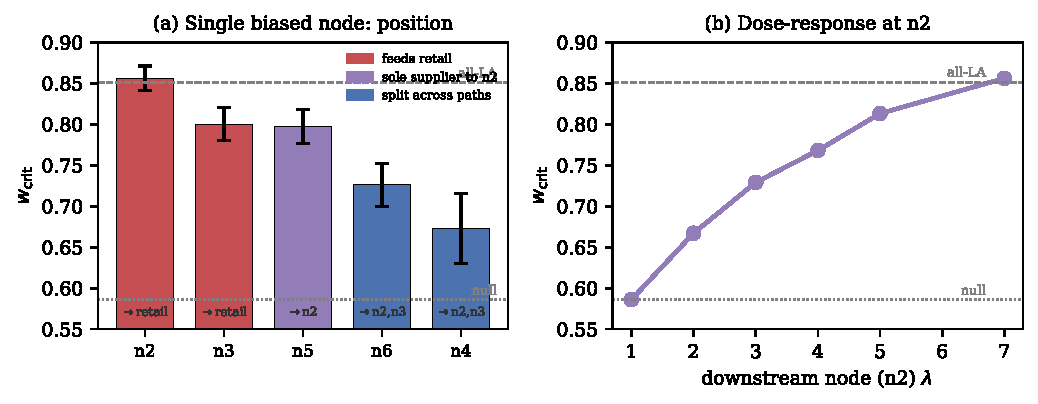
\includegraphics[width=\columnwidth]{Figures/cascade_tier_dose}
 \caption{A single loss-averse node can dominate the supply-chain boundary. (a)~One
  $\lambda{=}7$ node by position: the largest shifts come from nodes whose output reaches demand
  most directly, nodes feeding retail (red) dominate, the sole supplier to the dominant
  downstream node (purple) is comparable within noise to the second retail-feeder, and split-path
  suppliers (blue) are weaker as a group; CIs given in text above.
  (b)~Dose-response: increasing the downstream node's $\lambda$ moves $\wcrit$ monotonically up
  to the homogeneous all-loss-averse value ($0.854$, dashed).}
 \label{fig:s_cascade}
\end{figure}

\subsection{Deconfounding position with independent actors}
\label{sec:s_cascade_separate}
Because a single shared-parameter actor lets a biased node's gradient reach every other node
directly, the position ordering above is not by itself evidence that the effect is topological. We
designed a second sweep, identical in environment, $w$-grid, seeds, $\alpha,\beta,\lambda$, collapse
label, and estimator, but replacing the shared actor with five fully independent PPO models, one per
trainable node, each updated only on its own transitions and sharing no parameters or gradient.

\paragraph{Matching per-agent training exposure.} The shared actor's nominal $300$k
\texttt{total\_timesteps} is distributed across all $5$ agents by SuperSuit's
\texttt{pettingzoo\_env\_to\_vec\_env\_v1}, which packs the agents into one vectorized environment;
each individual agent therefore receives $\approx 300$k$/5=60$k real environment ticks of its own
transitions. To keep the two sweeps comparable, each independent actor in the separate-actor sweep is
trained for $60$k real ticks (round-robin in $2$k-step segments across $30$ rounds, each actor training
against the others' current, evolving policies), matching the shared actor's real per-agent exposure
rather than its nominal timestep count.

\paragraph{Result: the ordering is not topological.} Table~\ref{tab:s_cascade_separate} compares the
two sweeps directly. The ordering does not merely reshuffle: node\_2, the strongest position under the
shared actor ($\wcrit{=}0.863$, rank~1), is the \emph{weakest} of the five under separate actors
($\wcrit{=}0.498\,[0.363,0.581]$, rank~5), while node\_4, weakest under the shared actor, rises to
rank~2. The coarse retail-adjacent-vs-split-path grouping also fails to replicate: mean $\wcrit$ is
$0.832$ vs.\ $0.700$ (a clear gap) under the shared actor, and $0.606$ vs.\ $0.553$ (no longer cleanly
separated, and inverted by node\_2 alone) under separate actors. We conclude the position-specific
effect under the shared actor is substantially a shared-gradient artifact and do not draw a topological
reading from it.

\begin{table}[t]
\centering\small
\caption{Position sweep, shared vs.\ independent actors ($\lambda{=}7$, $n{=}20$/position/actor
condition, $2{,}000$-replicate seed-resampled bootstrap 95\% CI). Rank 1 = strongest effect on
$\wcrit$.}
\label{tab:s_cascade_separate}
\resizebox{\linewidth}{!}{%
\begin{tabular}{lcccc}
\toprule
Position & Shared $\wcrit$ & Rank & Independent $\wcrit$ & Rank \\
\midrule
node\_2 & $0.863\,[.846,.880]$ & 1 & $0.498\,[.363,.581]$ & 5 \\
node\_3 & $0.800\,[.780,.820]$ & 2 & $0.714\,[.683,.745]$ & 1 \\
node\_5 & $0.797\,[.740,.857]$ & 3 & $0.538\,[.474,.591]$ & 4 \\
node\_6 & $0.726\,[.682,.769]$ & 4 & $0.547\,[.495,.594]$ & 3 \\
node\_4 & $0.673\,[.622,.720]$ & 5 & $0.559\,[.502,.608]$ & 2 \\
\bottomrule
\end{tabular}%
}
\end{table}

% =======================================================================
\section{Two Boundary-Condition Ablations}
\label{sec:s_ablations}

\subsection{Action representation}
For the supply-chain base-stock control, the mechanism predicts that coarse discretization of the
scalar action representation can remove the near-boundary crossing.
Value-based learners need discrete actions, so we discretized the base-stock control into
$K{=}11$ bins and ran IQL and QMIX on the identical reward pipeline, $w$-grid, and label; both
produced a flat, $w$-independent collapse rate with no fittable $\wcrit$. To isolate the
cause, a single-variable control (PPO on the same $K{=}11$ discrete shell) also goes flat
(Table~\ref{tab:ablation_action}). At $K{=}11$, discretization \emph{alone} erases the boundary, so
the value-based nulls at that granularity need no appeal to the learning paradigm. This is not a
claim that discreteness per se removes the boundary: MPE is natively discrete and retains it. Coarse
bins snap the policy to a stable interior level and never visit the near-threshold $(s,S)$ region
where collapse occurs, consistent with the continuous-gradient account. We confirm only the $K{=}11$
point, not the shape of the boundary's dependence on $K$: we cannot currently distinguish
``coarseness of any granularity suppresses the boundary'' from ``the boundary specifically needs
near-continuous control, and would reappear at finer $K$.'' A granularity sweep
($K\in\{11,25,51,101\}$) on the supply-chain substrate would resolve this and is left to future work;
until then we report this as a substrate-specific, single-point scope condition, not a confirmed
general one.

\begin{table}[t]
\centering \small
\caption{Action-representation ablation at $K{=}11$ (the only granularity tested). The control
(last row) changes only the action space while holding the learner at PPO, isolating
discretization at this granularity, not the value-based paradigm, as what erases the boundary;
whether the boundary reappears at finer $K$ is untested.}
\label{tab:ablation_action}
\begin{tabular}{lll}
\toprule
Learner & Action space & Boundary? \\
\midrule
PPO / MAPPO & continuous & yes \\
QMIX (centralized value) & discrete $K{=}11$ & no \\
IQL (independent value) & discrete $K{=}11$ & no \\
PPO (control) & discrete $K{=}11$ & \textbf{no} \\
\bottomrule
\end{tabular}
\end{table}

\subsection{Credit assignment}
The boundary is measurable only with a learner that can coordinate on a shared-reward task.
On MPE, independent PPO never reaches the coordinated regime at \emph{any} $w$ (collapse
fraction $1.0$ throughout, including maximal centralization; Figure~\ref{fig:mpe_floor}), so
collapse induced by the reward transform cannot be distinguished from inability to assign credit. Centralized-critic
MAPPO recovers coordination (collapse fraction falls to $0.35$, occupancy crosses the threshold
near $w\approx0.6$). The same floor appears on LBF. The boundary is therefore measurable on these
shared-reward tasks only with a centralized critic. Matching MAPPO to such environments is a
necessity, not a convenience.

\begin{figure}[t]
 \centering
 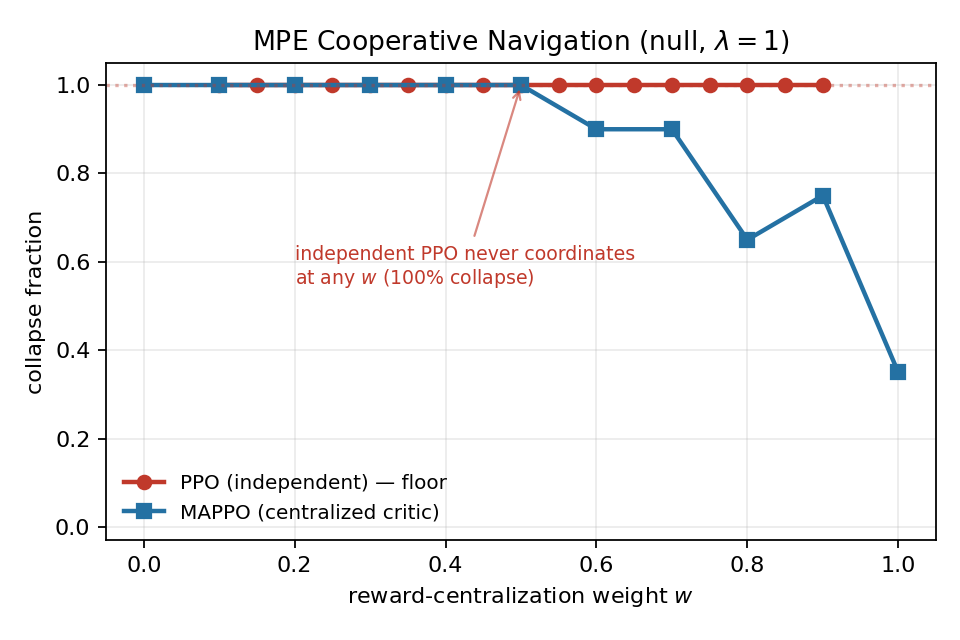
\includegraphics[width=0.9\columnwidth]{Figures/mpe_ppo_coordination_floor}
 \caption{Credit-assignment ablation on MPE (null, $\lambda{=}1$). Independent PPO collapses
  at every $w$ (a coordination floor), while centralized-critic MAPPO crosses the boundary.
  The reward-transform boundary is exposed only once credit assignment is handled.}
 \label{fig:mpe_floor}
\end{figure}

% =======================================================================
\section{Pre-registered Signal-to-Noise Probe}
\label{sec:s_snr}

The mean-field account calibrates the magnitude of $\wcrit$ rather than predicting it, because the
drift and diffusion coefficients are properties of the stochastic PPO learning dynamics. We
pre-registered a direct measurement intended to test whether these coefficients could localize the
boundary. During PPO training we logged the policy mean once per update and, over a fixed early
window, estimated an empirical drift $\widehat F(w)$ from mean increments and an empirical diffusion
variance $\widehat\Sigma(w)$ from increment variance. We formed
\begin{equation}
 \widehat{\mathcal S}(w)=\frac{\widehat F(w)}{\sqrt{\widehat\Sigma(w)}} .
\end{equation}
If one uses the alternative convention $\Sigma=2\Theta$, the constant factor is absorbed into the
critical threshold and does not change any crossing or sign claim. \textbf{Boundary-reproduction
check:} sweep $w\in\{0.50,\dots,0.90\}$ at the structural condition, 20 seeds/$w$, 150k steps; the
measured collapse-fraction crossing should reproduce the matched-horizon boundary
$\wcrit=0.822$. \textbf{Outcome (reported in full):} the collapse-fraction of this
independent sweep crosses $0.5$ at $w=0.82$, reproducing the matched-horizon boundary almost
exactly, a positive robustness check on the boundary. The \emph{drift-sign} observable,
however, was \emph{inconclusive}: the restoring drift in the contested band is weakly positive
across all $w$ with no genuine zero-crossing, so it does not localize $\wcrit$. The reason is
basin geometry, PPO initializes above the cooperative optimum ($S{\approx}250$ vs
$S{\approx}150$), and collapses plunge through the contested band too quickly to sample,
biasing the conditioned drift toward survivors.

\textbf{Non-survivor-biased re-probe (also negative).} We tested the natural fix directly. We
re-ran the identical sweep with the policy re-initialized at the cooperative optimum
($S{\approx}150$, actor mean biased to $a_0{=}{-}0.4$) so that both surviving and collapsing runs
are sampled inside the contested band during early training, and added a second,
initialization-robust \emph{basin-flow} localizer (net early displacement of the policy mean from
the optimum) alongside the restoring-drift statistic. The re-initialization de-biased the
observable (the drift is now smooth and monotone in $w$ rather than flat and noisy) and the
collapse-fraction crossing again reproduced the boundary ($\wcrit\approx0.83$). But neither
statistic \emph{localizes} $\wcrit$: the drift and basin-flow are monotone in $w$ without a
zero-crossing, and their steepest change falls near $w{\approx}0.6$, not at the boundary. The
observable therefore tracks \emph{where the policy sits} rather than \emph{where the boundary is},
which the initialization change does not fix. We consequently report magnitude localization as
genuinely open: the sign-level account and single-substrate functional-form summary remain useful,
but a magnitude-level prediction of $\wcrit$ remains future work. The re-probe driver and analysis are
released with the code.

% =======================================================================
\section{Exploration-Noise Ablation}
\label{sec:s_entropy}

The SNR account predicts that injected exploration noise raises $\wcrit$ when it is the binding
SNR term. Sweeping the PPO entropy coefficient at the structural condition (300k, 20 seeds,
$w\in\{0.5,\dots,0.9\}$), the supply-chain boundary rises monotonically:
$\wcrit=0.685$ at $\text{ent}{=}0$ (reproducing the null), $0.690$ at
$0.001$, $0.715$ at $0.01$, and beyond $0.05$ the system collapses at every tested $w$
(Table~\ref{tab:entropy}). \textbf{A binding-noise dissociation.} Repeating under MAPPO on the
transfer substrates: on LBF the prediction replicates ($\wcrit$ rises $0.13\to0.37$ over
$\text{ent}\in\{0,0.05\}$, shift $+0.24$, non-overlapping endpoints); on MPE the boundary does
\emph{not} move (shift $+0.05$, overlapping CIs; pooled slope over 1{,}320 runs positive but
not significant, $\beta{=}{+}0.47$, CI $[-3.4,+4.3]$). This is a dissociation predicted by the
mechanism: exploration noise moves the boundary only when it is the binding term in the SNR.
The supply chain and LBF have sparse, sharp landscapes where injected entropy dominates; MPE's
dense distance-shaped reward carries high intrinsic exploration that swamps the added term. The
pattern matches the binding-noise criterion: the boundary moves where injected entropy is binding
and is statistically flat where it is not.

\begin{table}[t]
\centering \small
\caption{Entropy-coefficient ablation ($\alpha{=}\beta{=}1$, $\lambda{=}1$, 300k, 20
seeds/cell). $\wcrit$ with bootstrap 95\% CIs.}
\label{tab:entropy}
\begin{tabular}{cc}
\toprule
entropy coef. & $\wcrit$ (95\% CI) \\
\midrule
0.000 & 0.685 [0.656, 0.710] \\
0.001 & 0.690 [0.667, 0.715] \\
0.010 & 0.715 [0.689, 0.743] \\
0.050 & $>1$ (collapse at all $w$) \\
\bottomrule
\end{tabular}
\end{table}

\begin{figure}[t]
 \centering
 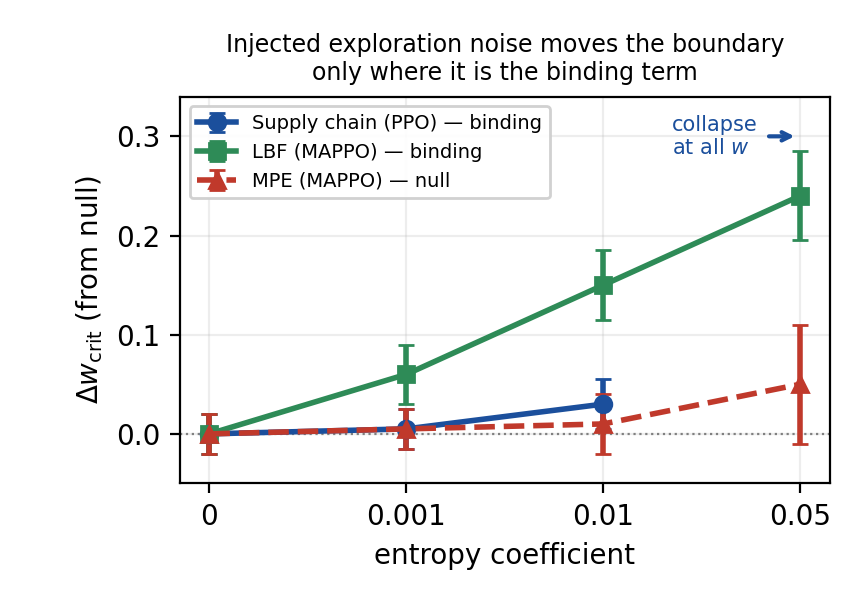
\includegraphics[width=0.82\columnwidth]{Figures/entropy_dissociation.png}
 \caption{Entropy-ablation dissociation across substrates. Injected exploration noise raises $\wcrit$
  clearly on LBF (non-overlapping CIs); the supply-chain shift is same-direction but within noise
  (overlapping CIs); MPE is flat, where dense-reward intrinsic exploration dominates.}
 \label{fig:dissociation}
\end{figure}

% =======================================================================
\section{Threshold Robustness}
\label{sec:s_robustness}

We re-estimate $\wcrit$ on Exp~A @300k under nine variants of the collapse definition, varying
the $\bar S$ threshold over $\{8,10,12\}$ and the $\bar\pi$ threshold over
$\{-102.5,-127.1,-152.5\}$. Three variants with $\bar\pi\le-152.5$ are degenerate (the minimum
profit in the dataset is $-128.1$) and excluded. Across the remaining six estimable variants
the maximum deviation from the baseline $\wcrit=0.666$ is $0.015$, well below the CI width: the
collapse definition is robust to $\pm20\%$ threshold perturbation.

% =======================================================================
\section{Reward-Transform Controls}
\label{sec:s_controls}
The loss-aversion treatment also changes reward magnitude, variance, and (through the fixed zero
reference) the gain/loss split. We isolate these with three matched controls on the supply chain,
holding the environment, PPO configuration (\S\ref{sec:s_setup}), $w$-grid, seeds (42--61), and
collapse label fixed; only the named factor moves. Reference points and the RMS scale were measured
on $\lambda{=}1$ (untreated) data and frozen before the sweeps (pre-registration records released with
the code).

\paragraph{What ``same seed'' means, and paired vs.\ unpaired uncertainty.} The paired-bootstrap
comparison depends on what is actually shared between two runs carrying the same integer seed $s$, since assigning a
common label does not by itself make observations statistically paired. In our driver, $s$ sets three
things jointly: the PPO network's parameter initialization (\texttt{PPO(..., seed=s)}), the
environment's reset/transition RNG stream, and the evaluation episode seeds (deterministic functions
of $s$). So seed-$s$ runs across $w$-cells and $\lambda$ arms start from the same initial weights and
draw from the same underlying randomness stream, not merely a shared bookkeeping label; treating $s$ as
the resampling unit (a block/cluster bootstrap) is the standard practice this justifies. The bootstrap
resamples whole seeds with replacement, $2{,}000$ replicates; every reported difference (across
$\lambda$ or control arm) draws the \emph{same} resampled seed multiset for both endpoints within a
replicate (seed-paired), which is what lets us separate evaluation-episode noise from training-seed
noise for the difference specifically.

To check whether pairing is understating uncertainty, we also computed an
\emph{unpaired} version: the two endpoints are resampled independently, so cancellation from shared
resampling noise cannot occur. For the same endpoint convention as the main-paper generalization table,
the paired shifts are supply chain
$+0.269$, MPE $+0.11$, and LBF $+0.57$ (using LBF's last interior endpoint, $\lambda{=}4$, rather than
the ceiling-extrapolated higher-$\lambda$ fits). The unpaired check gives the same signs and only
marginally wider intervals, so pairing is not materially shrinking the reported conclusions.

\emph{Control~A (reference point).} The value transform is not invariant to adding a constant, so we
re-run $\lambda\in\{1,3,7\}$ with the gain/loss reference $z_0$ shifted to four frozen values and
re-anchor $v(x-z_0)$. \emph{Control~B (scale match).} We divide the transformed reward by a
per-$\lambda$ constant equal to its RMS relative to $\lambda{=}1$ (measured RMS $7.93,17.06,31.87$ at
$\lambda{=}1,3,7$), matching magnitude across conditions. \emph{Control~C (reward units).} We multiply
the local, or the team, reward by $2$ before blending, changing the nominal-to-effective mixing ratio.

\begin{table}[t]\centering\small
\caption{Reward-transform controls (supply chain, PPO, 300k, 20 seeds). Shift is the seed-paired
$\lambda{=}1{\to}7$ change in $\wcrit$ (Firth); CI = 2{,}000-resample paired bootstrap. Baseline
(reference $0$, unit scale) shift is $+0.269$ $[0.232,0.306]$.}
\label{tab:s_controls}
\setlength{\tabcolsep}{4pt}
\resizebox{\linewidth}{!}{%
\begin{tabular}{@{}llcc@{}}
\toprule
Control & Arm & $\wcrit(\lambda{=}1)$ & Shift $\lambda{=}1{\to}7$ \\
\midrule
A ref.\ point & $z_0={-}2.99$ (mean)   & 0.605 & $+0.228\,[0.187,0.272]$ \\
A ref.\ point & $z_0={-}6.77$ (median) & 0.626 & $+0.183\,[0.122,0.269]$ \\
A ref.\ point & $z_0={-}5.14$ ($-0.5\sigma$) & 0.621 & $+0.193\,[0.141,0.247]$ \\
B scale match & RMS-matched            & 0.585 & $+0.145\,[0.107,0.185]$ \\
C reward unit & $2\times$ local        & 0.779 & $+0.130\,[0.105,0.153]$ \\
C reward unit & $2\times$ team         & 0.476 & $+0.329\,[0.263,0.430]$ \\
\bottomrule
\end{tabular}%
}
\end{table}

Reading: the $\lambda{=}1{\to}7$ shift is positive with a zero-excluding CI in every arm of A and B
and in all three arms of C, so it is not an artifact of the reference point or of reward
magnitude/variance. In C the absolute $\wcrit$ moves ($+0.194$ at $\lambda{=}1$ under $2\times$ local,
$-0.109$ under $2\times$ team), confirming that $w$ is a nominal mixture coefficient whose numerical
boundary is conditional on reward parameterization.

\paragraph{The incentive ratio $\varrho$, reported numerically.} The main paper uses
$\varrho=(1-\wcrit)c_\ell/(\wcrit c_g)$ as the coordinate-adjusted quantity; here we report its
value directly from Control C, where $c_\ell,c_g$ are the pre-registered
reward-unit multipliers of that arm ($c_\ell{=}2,c_g{=}1$ for $2\times$ local; $c_\ell{=}1,c_g{=}2$ for
$2\times$ team; $c_\ell{=}c_g{=}1$ at baseline), using the same Firth $\wcrit$ and seed-resampling
bootstrap as elsewhere (\texttt{experiments/compute\_varrho.py}, reads existing Control C data, no new
training).

\begin{table}[t]\centering\small
\caption{Incentive ratio $\varrho=(1-\wcrit)c_\ell/(\wcrit c_g)$ by Control C arm and $\lambda$.
Bootstrap 95\% CI, 2{,}000 seed resamples.}
\label{tab:s_varrho}
\begin{tabular}{llccc}
\toprule
Arm & $c_\ell,c_g$ & $\lambda$ & $\wcrit$ & $\varrho$ (95\% CI) \\
\midrule
Baseline    & $1,1$ & 1 & 0.585 & $0.710\,[0.596,0.836]$ \\
Baseline    & $1,1$ & 3 & 0.775 & $0.291\,[0.266,0.325]$ \\
Baseline    & $1,1$ & 7 & 0.854 & $0.171\,[0.148,0.195]$ \\
$2\times$ local & $2,1$ & 1 & 0.779 & $0.568\,[0.500,0.651]$ \\
$2\times$ local & $2,1$ & 3 & 0.880 & $0.272\,[0.222,0.306]$ \\
$2\times$ local & $2,1$ & 7 & 0.909 & $0.200\,[0.175,0.222]$ \\
$2\times$ team  & $1,2$ & 1 & 0.476 & $0.550\,[0.449,0.798]$ \\
$2\times$ team  & $1,2$ & 3 & 0.726 & $0.189\,[0.167,0.214]$ \\
$2\times$ team  & $1,2$ & 7 & 0.805 & $0.121\,[0.098,0.145]$ \\
\bottomrule
\end{tabular}
\end{table}

$\varrho$ is \emph{not} itself invariant across arms at fixed $\lambda$: at $\lambda{=}1$ the three arms
give $0.710$, $0.568$, $0.550$, a spread of $0.16$ with CIs that overlap but are not coincident, so
$\varrho$ under this nominal (unit-multiplier) definition does not fully absorb the reward-unit change.
It is, however, tighter than the raw boundary: at $\lambda{=}1$ the reward-unit spread in $\wcrit$
itself is $0.30$ ($0.780$ to $0.476$ across the two $2\times$ arms), roughly twice $\varrho$'s spread of
$0.16$; the compression ratio is $0.53$ at $\lambda{=}1$, weakening to $0.66$ at $\lambda{=}3$ and
$0.76$ at $\lambda{=}7$ (Table~\ref{tab:s_varrho}), so $\varrho$ is a partial, not complete, correction
that degrades somewhat as $\lambda$ grows. What does hold, in every arm without exception, is the
\emph{direction}: $\varrho$ falls monotonically from $\lambda{=}1$ to $\lambda{=}7$, by a comparable
relative amount ($-76\%$ baseline, $-65\%$ $2\times$ local, $-78\%$ $2\times$ team), so the
loss-aversion shift is not an artifact of the reward-unit convention even though $\varrho$'s absolute
level is convention-dependent. We considered
whether an RMS-based (measured, rather than nominal multiplier) definition of $c_\ell,c_g$ would rescue
full invariance, but the pre-blend local and global reward streams were not separately logged during
Control C's runs (only the post-blend value was recorded), and no model checkpoints were retained, so
testing this would require a new training sweep rather than reanalysis; we leave it to future work and
report the nominal-scale result here without overstating it.

% =======================================================================
\section{Notation and Abbreviations}
\label{sec:s_notation}

\begin{table}[h]
\centering \small
\begin{tabular}{lp{0.62\linewidth}}
\toprule
Symbol & Meaning \\
\midrule
$w$ & reward centralization weight, $\in[0,1]$ \\
$\wcrit$ & critical $w$ where $P(\mathrm{collapse}){=}0.5$ \\
$\lambda$ & loss-aversion coefficient ($\lambda{>}1$) \\
$\alpha,\beta$ & prospect-theoretic value-function curvature (gain/loss) \\
$\rho$ & loss-domain share of marginal incentive, $\in[0,1]$ \\
$g,c$ & marginal global benefit / local cost of cooperation \\
$F,\Sigma$ & policy-mean drift / stochastic-update diffusion variance \\
$\mathcal{S}(w,\lambda)$ & $F_{\mathrm{esc}}/\sqrt{\Sigma_{\mathrm{esc}}}$, escape signal-to-noise ratio \\
$\sigma,\eta,B$ & exploration scale / learning rate / batch size \\
$\Delta U,\tau$ & escape barrier / Kramers first-passage time \\
$T$ & training horizon (environment steps) \\
$\bar S,\bar\pi$ & mean base-stock / mean profit (collapse label) \\
\bottomrule
\end{tabular}
\end{table}

\noindent\textbf{Abbreviations.} MARL (multi-agent reinforcement learning); CTDE (centralized
training, decentralized execution); PT value transform (prospect-theoretic value transform); PPO (proximal policy
optimization); MAPPO (multi-agent PPO with a centralized critic); MPE (multi-agent particle
environments); LBF (Level-Based Foraging); SNR (signal-to-noise ratio); CI (confidence
interval).

% =======================================================================
\section{Claim--Evidence Ledger}
\label{sec:s_ledger}

Table~\ref{tab:claim_ledger} assigns each headline claim to its evidence bucket. The loss-aversion
direction is the generalizing core; the curvature sign, affine law, and downstream-minority cascade
are supply-chain-specific unless separately replicated.

\begin{table}[h]
\centering \small
\caption{Claim ledger after the final scope pass. SC = supply chain.}
\label{tab:claim_ledger}
\begin{tabular}{p{0.42\linewidth}p{0.44\linewidth}}
\toprule
Claim & Evidence bucket \\
\midrule
Sharp collapse boundary $\wcrit$ exists & measured generally (SC, MPE, LBF; PPO/MAPPO) \\
Metastability: $\wcrit$ slides with $T$ & measured generally (SC, MPE, LBF; PPO/MAPPO) \\
Loss aversion raises $\wcrit$ & measured generally for direction (SC, MPE, LBF; PPO/MAPPO) \\
Curvature lowers $\wcrit$ & measured only on SC PPO; not universal \\
Affine $\lambda$-law & calibrated/fitted on SC PPO only \\
Mean-field sign account & modeled/sign-level under SC PPO SNR premise \\
Downstream-minority cascade & measured only on SC PPO; future work for other directed-flow domains \\
Closed-form numerical $\wcrit$ & future work \\
\bottomrule
\end{tabular}
\end{table}

% =======================================================================
\bibliography{references}

\end{document}
